\section{A motivating example: Parkinson's disease}
\label{intro-complete_ex}

As a motivating example, we now turn to the descriptive
epidemiological metaregression of Parkinson's disease (PD). A
systematic review of PD was conducted as part of the GBD 2010
Study.\cite{TK_GBD_2010_or_parkinsons_paper} The results of this
review---data on the prevalence, incidence, and standardized mortality ratio of
PD---needed to be combined to produce estimates of disease prevalence by
region, age, sex, and year.  These prevalence estimates were combined
with disability weights to measure years lived with disability (YLDs),
which were then combined with estimates of years of life lost (YLLs)
to produce estimates of the burden of PD quantified in disability-adjusted life-years (DALYs).

PD is a neurodegenerative disorder that includes symptoms of motor
dysfunction, such as tremors, rigidity, and akinesia, in the early
stages of the disease.  As the disease develops, most patients also
develop nonmotor symptoms, such as cognitive decline, dementia,
autonomic failure, and disordered sleep-wake regulation.  The standard
definition for PD diagnosis includes at least two of four cardinal
signs---resting tremor, bradykinesia, rigidity, and postural abnormalities.
There is no cure or treatments to slow the progression of the disease;
however, motor symptoms and disability may be improved with
symptomatic therapy.\cite{poewe_natural_2006, pollock_prevalence_1966, larsen_clinical_1994}

Systematic review for PD yielded $782$ data points that met the inclusion criteria: $660$
prevalence, $99$ incidence, and $13$ standardized mortality ratio data
points.  A separate analysis of
mortality due to PD was carried out as part of the GBD 2010 Study and
provided $1638$ additional data points of cause-specific mortality by
region, age, and sex for the years 1990, 2005, and 2010.  Prevalence
is measured as a percent, standardized mortality ratio is a unitless number, and
incidence and cause-specific mortality is measured in $10,000$ person
years (PY).  It is important to note that in this example, cause-specific mortality means
that the person issuing a death certificate deemed the person to
have died \emph{from} the disease as the underlying cause and not
simply \emph{with} it.  This subtle distinction is elaborated on in
section~\ref{theory-csmr} and demonstrated further in
chapter~\ref{applications-csmr}.

Even when restricting the data to a
specific geographic region, such as Western Europe, the data remain
noisy and heterogeneous, as seen in figure~\ref{fig:intro-parkinsons
  data}. This figure shows a horizontal bar for each data point, where
the left and right endpoints depict the start and end ages of the age
interval measured, and the position of the bar on the $y$-axis indicates the value of the
measurement. Section~\ref{theory-age_group_model-overlapping_data}
describes our approach to making
robust estimates in the face of such heterogeneous levels and
overlapping age groups.

    \begin{figure}[h]
        \begin{center}
            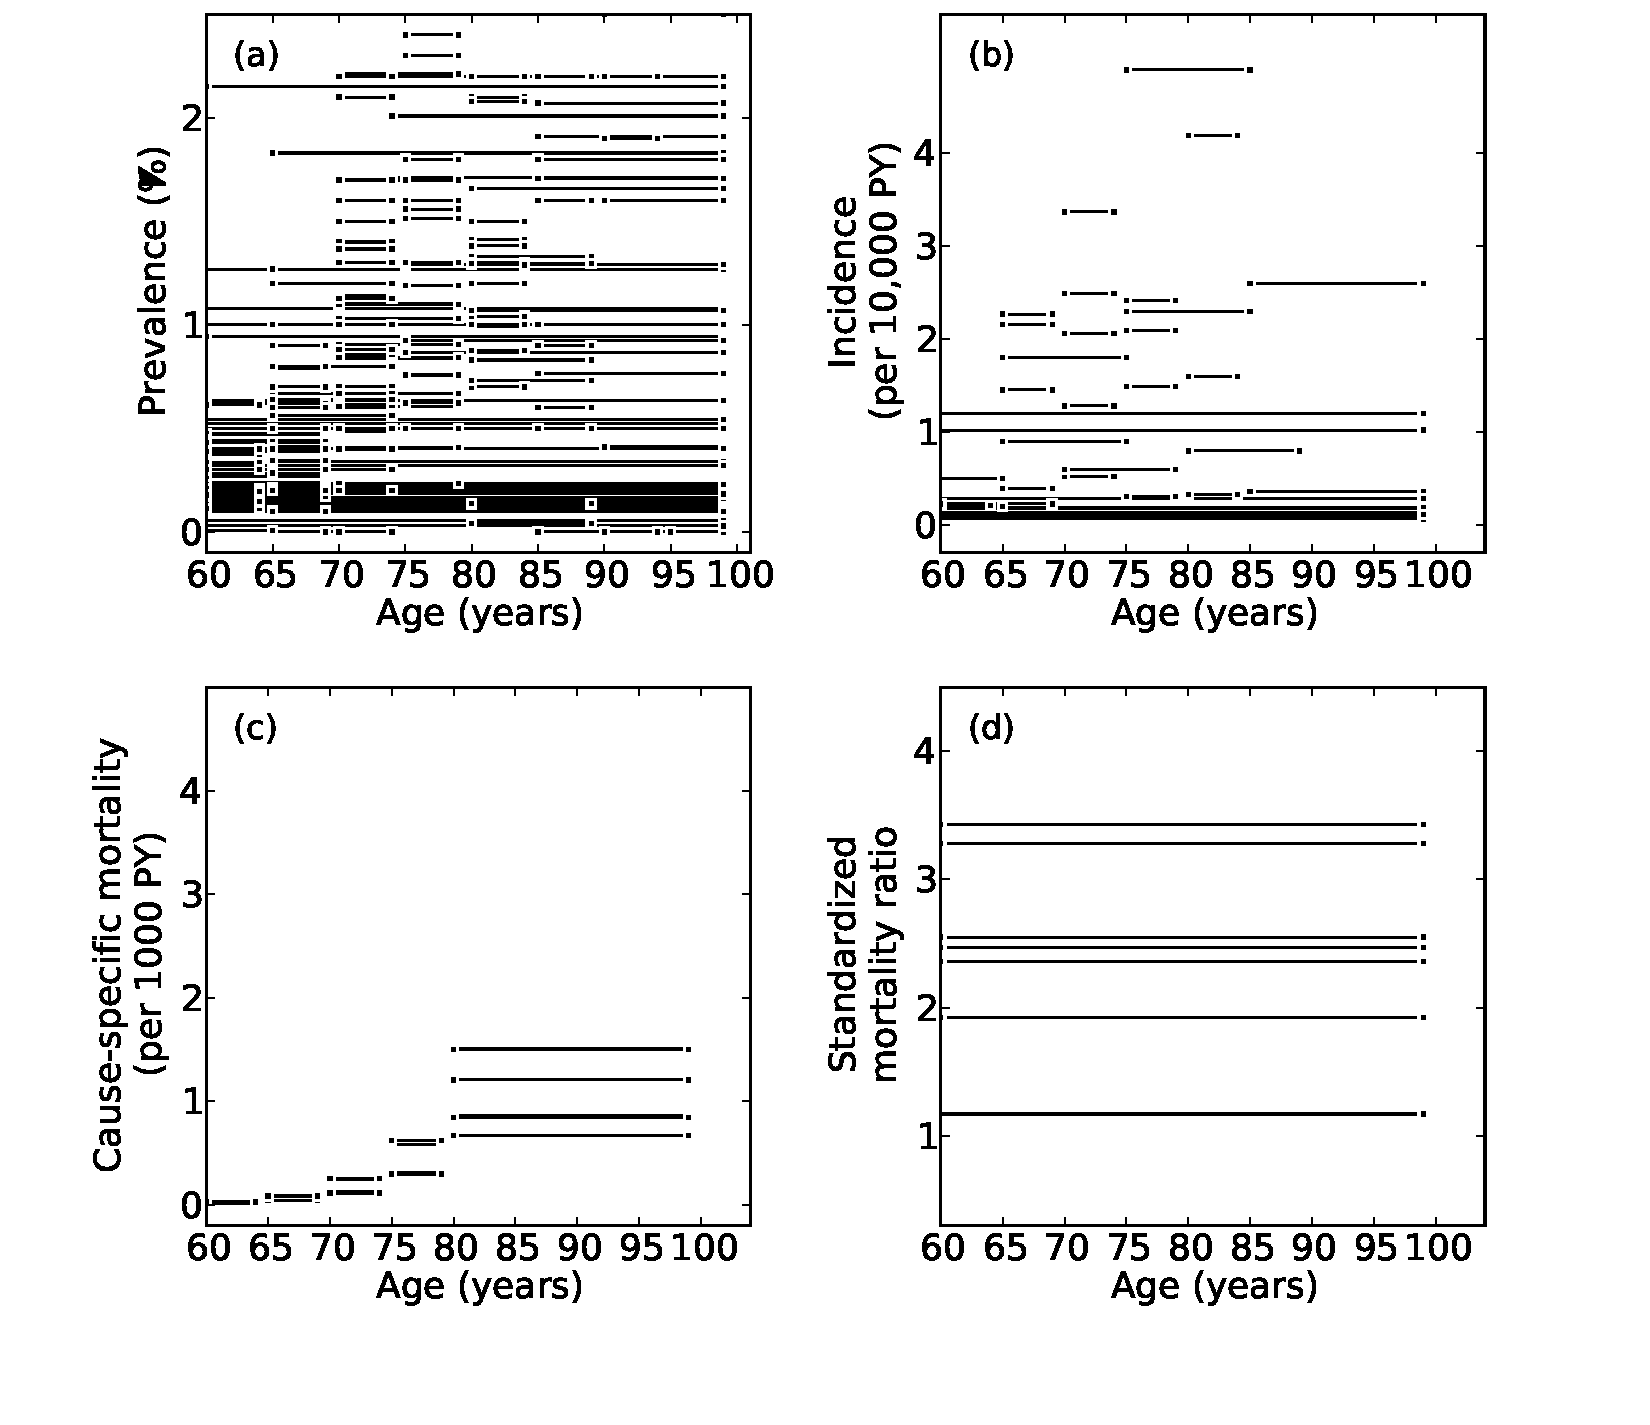
\includegraphics[width=\textwidth]{parkinsons-data.pdf}
            \caption[Systematic review data for Parkinson's disease.]{Data points from systematic review of descriptive
              epidemiology of Parkinson's disease, showing data from
              Western Europe on (a) prevalence, (b) incidence, (c)
              cause-specific mortality, and (d) standardized mortality
              ratio.}
            \label{fig:intro-parkinsons data}
        \end{center}
    \end{figure}

The data points represent the results
of many different studies conducted for many different reasons over the last $50$ years.
Study-level fixed effects, discussed in chapter
~\ref{theory-covariate_modeling} and demonstrated further in
chapter~\ref{applications-efx_study_level}, aid the model in
explaining bias resulting from differing diagnostic criteria and study
populations.  The model finds no more bias associated with subnational
studies than with national studies, estimating that the former are
shifted in log-space by $-0.03$ on average, with a 95\% uncertainty
interval (UI) of $[-1.1, 1.2]$.  Similarly, the model estimates that studies that did not use a
neurologist are shifted in log-space by $0.02$ with a
UI of $[-0.3, 0.3]$.  Studies that used a nonstandard definition for PD
diagnosis, on the other hand, were found to be systematically biased
to lower levels of prevalence than studies using a standard definition. The
effect coefficient for the shift in log-space was estimated to have a
mean of $-0.48$ and a UI of $[-0.7, -0.2]$.

Of the $21$ regions reported in the GBD 2010 Study, only $36$ countries
from $16$ regions are represented in the systematic review of PD.  The GBD
2010 Study predicts year-age-sex estimates for all countries, even
those without data.  To predict out-of-sample year-age-sex estimates, country-level random
effects provide a solution to the problem of missing epidemiological data,
as developed in chapter~\ref{theory-covariate_modeling}.  The model for PD uses the
kilocalories of stimulants consumed per capita per day and national smoking prevalence
as country-level covariates.  For an increase of one unit of stimulants per
capita per day, the model estimates a shift in log-space of $-0.34$
with a UI of $[-0.5, -0.2]$.  Similarly, for an increase of one unit in national
smoking prevalence, the model predicts a shift in log-space of $-0.02$ with a UI
of $[-0.05, -0.01]$.

Nonsampling variation that cannot be explained is another problem with
such noisy and heterogeneous data.  Chapter~\ref{theory-covariate_modeling}
explains how random effects can be used
to estimate the systematic differences between countries within a
region, regions within a superregion, and so on.  Since this example
contains data from Western Europe only, it is the country-level random
effects that are relevant here.  For example, the model estimates that
prevalence in the Netherlands is above the regional mean, shifting
estimates up by $20\%$ (UI $[0, 50]$\%).  The model also estimates
that prevalence in Great Britain is below the regional mean, shifting estimates
down by $15\%$ (UI $[0, 30]\%$).

It is intuitive that there is a relationship between the
different epidemiological parameters: every prevalent case was once an incident
case, for example.  Combining all parameters to produce internally
consistent results is discussed in detail in section~\ref{sys-dynamics}.
Through the process of data confrontation
discussed in the following chapters, the meta-analysis produces a best
estimate and uncertainty bounds of disease prevalence, as shown in
figure~\ref{fig:intro-parkinsons fit}.

    \begin{figure}[h]
        \begin{center}
            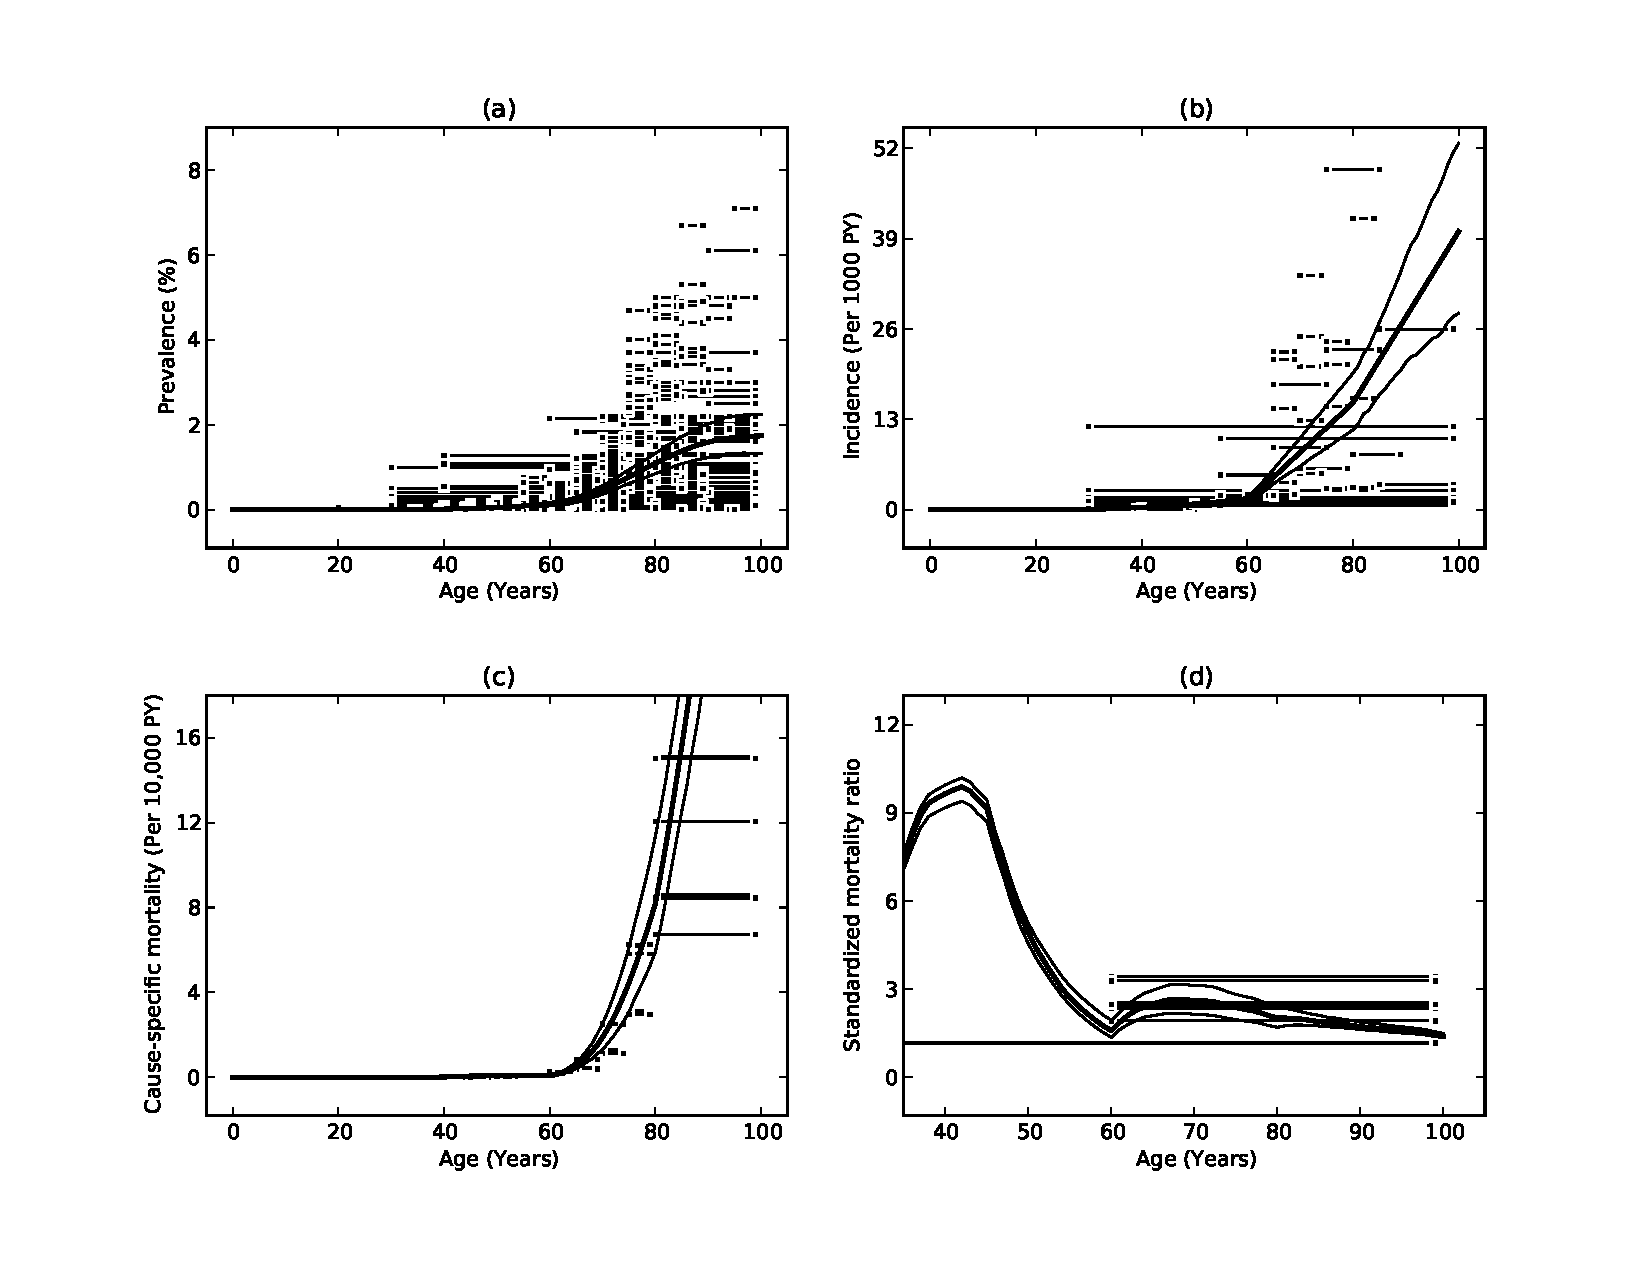
\includegraphics[width=\textwidth]{parkinsons-best.pdf}
            \caption[Estimates of age-specific rates for Parkinson's disease.]{Estimates
              of age-specific rates of
              (a) prevalence, (b) incidence,
              (c) cause-specific mortality, and
              (d) standardized mortality ratio of Parkinson's
              disease in Western European females in 2005.}
            \label{fig:intro-parkinsons fit}
        \end{center}
    \end{figure} 